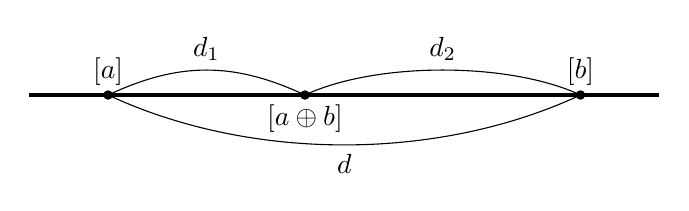
\begin{tikzpicture}
  \coordinate (A) at (1, 0);
  \coordinate (B) at (7, 0);
  \coordinate (P) at (3.5, 0);
  
  \draw[very thick] (0, 0) -- (8, 0);
  \filldraw[black] (A) circle (1.5pt) node[anchor=south] {$[\vc {a}]$};
  \filldraw[black] (B) circle (1.5pt) node[anchor=south] {$[\vc {b}]$};
  \filldraw[black] (P) circle (1.5pt) node[anchor=north] {$[\vc {a} \oplus \vc {b}]$};
  
  \draw (A) to [out=25, in=155, distance=1cm] node[midway, above] {$d_1$} (P);
  \draw (P) to [out=25, in=155, distance=1cm] node[midway, above] {$d_2$} (B);
  \draw (A) to [out=155, in=25, distance=-2cm] node[midway, below] {$d$} (B);
\end{tikzpicture}
